\chapter{Números de máquina y número de condición}
\setcounter{equation}{0}
\section{Cuestiones previas}

En el \emph{álgebra lineal computacional} (o en el análisis numérico en general) interesan no solo los algoritmos sino su \emph{confiabilidad}  y su \emph{costo computacional}. La primera cuestión aparece porque en la práctica no es posible en general trabajar con precisión infinita (lo que hace imprescindible el  estudio de los errores numéricos y su propagación). La segunda cuestión tiene que ver con el número de operaciones involucradas en el algoritmo (\emph{complejidad del algoritmo}) cuestión que impacta en el tiempo de ejecución\footnote{Otras consideraciones son posibles: por ejemplo si puede o no paralelizarse.}.

Comenzamos entonces definiendo de manera informal los números de máquina.
\tcc
Los números de máquina, son los que la máquina puede representar de forma exacta.
\etcc
Notemos que -por su propia definición- podemos sospechar que los números de máquina son finitos y en consecuencia la \emph{mayoría} de los números reales no podrán almacenarse sin cometer errores. Vamos a tratar de precisar este punto en lo que sigue. Vamos a asumir que trabajaremos con número reales o complejos, sin embargo como para almacenar un número complejo basta almacenar su parte real e imaginaria podemos enfocarnos en el caso real.

Consideremos un número cualquiera, por ejemplo $x=125.4$. Estamos habituados a trabajar en base 10 lo que significa que estamos pensando a $x$ en la forma
$$
x=1\,10^2+2\,10^1+5\,10^0+4\,10^{-1}.
$$
Para número real (positivo) diferente, la escritura
$$
\bt_k\bt_{k-1}...\bt_0.\bt_{-1}\bt_{-2}...
$$
con $0\le \bt_i\le 9$ y $\bt_k\neq 0$, la asociamos con
$$
x=\sum_{-\infty}^k \bt_{i}10^{i}.
$$
La escritura hecha de este modo es \'unica, salvo desarrollos periódicos del número $9$ como ocurre en el caso
$$
0.999...=1,
$$
en el que el mismo número, en este caso $x=1$, puede escribirse de dos modos distintos.
En este contexto, el número $10$ se denomina la base y los $\bt_i$ los dígitos del desarrollo.
\section{Bases generales*}
En general todo número  $x\in \R$ $x\neq 0$, puede representarse en una base $b\in\N$, $b\ge 2$, de la forma\footnote{$(x)_b$ se lee $x$ en la base $b$.}
\begin{equation}
 \label{eq:represbaseb}
(x)_b=sg(x)\bt_k\bt_{k-1}...\bt_0.\bt_{-1}\bt_{-2}...
 \end{equation}
donde los ``dígitos'' verifican $0\le \bt_i\le b-1$, $sg(x)$ el signo de $x$ y donde por convención numeramos los índices para que el punto -o coma- se ubique entre $\bt_0$ y $\bt_{-1}$.

Asumamos que $x$ es positivo para no lidiar con el signo. La representación \eqref{eq:represbaseb} se obtiene de la escritura de $x$ como
$$
x=\bt_kb^k+\bt_{k-1}b^{k-1}+...+\bt_0b^0+\bt_{-1}b^{-1}+\bt_{-2}b^{-2}+...
$$
 que es única si  descartamos los desarrollos infinitos de la forma $\bt_j=b-1$ para todo $j\le l$ con $l\in \Z$ fijo.

 Para aclarar este punto recordemos la expresión  cerrada de la geométrica
$$
\sum_{j=0}^m\beta^j=\frac{\beta^{m+1}-1}{\beta -1},
$$
 válida para $\beta\neq 1$. Notemos que  en caso de tener un $x$ con un desarrollo de la forma
$$
x=\sum_{i=-\infty}^l(b-1)b^i,
$$
podemos reescribirlo como
$$
x=(b-1)b^{l}
\left(\sum_{i=-\infty}^0b^i\right)=(b-1)b^l\frac{b}{b-1}=b^{l+1},
$$
lo que indica dos  representaciones alternativas para el mismo $x$. Como ejemplo si  $l=0$ tenemos
$$
10=(x)_b=(b-1).(b-1)(b-1)(b-1)\cdots
$$

Continuemos asumiendo que $x>0$. El uso del punto \emph{fijo} en  \eqref{eq:represbaseb}  determina la división entre su \emph{parte entera}\footnote{La parte entera de $x$, denotada $[x]$ se define como el mayor entero menor o igual a $x$.}  $[x]\in \Z$ y la diferencia $0\le x-[x]<1$. En efecto, por un lado, para todo $m\in \N$
$$\sum_{0}^m\bt_i b^i\in \Z$$
y
$$
0\le \sum_{-\infty}^{-1}\bt_ib^{i}<\sum_{-\infty}^{-1}\bt_i(b-1)=(b-1)\frac{1}{b-1}=1.
$$
Por otro lado, esta representación tradicional no da una idea rápida del orden de magnitud
de un número. Por esta razón se suele trabajar con una versión \emph{normalizada}  eligiendo ubicar el punto justo a la izquierda de $\bt_k$ (i.e. el primer dígito no nulo de $x$). Así, un $0\neq x\in \R$, puede escribirse (renombramos los dígitos eliminando el tilde y los índices)

\begin{equation}
 \label{eq:notcientnorm}
(x)_b=sg(x) \, 0.b_0b_1b_2...\, b^{e}
\end{equation}
donde, como antes, $0\le b_i\le b-1$ y $e\in \Z$.
Una vez más, esta representación es única si asumimos que $b_0\neq 0$, y que en el caso $b_i=b-1$ para $i\le l$, $b_{i+1}<b-1$
convenimos en tomar
$$
(x)_b=sg(x)\, 0.b_0b_1...(b_{i-1}+1)\, b^{e+1}.
$$
Suele llamarse notación científica normalizada a la escritura \eqref{eq:notcientnorm}. La expresión  $0.b_0b_1b_2...$ se llama \emph{mantisa} y $e$  \emph{exponente}. Con esta normalización se ve a simple vista que $b^e< x\le b^{e+1}$.

Observemos que el exponente es un entero que admite asimismo una representación en la misma base $b$
$$e=sg(e)\, c_lc_{l-1}...c_{0}$$
donde una vez mas $c_l\neq 0$ y
$e=sg(e)\, \sum_0^{l}c_ib^i$.

\section{Números de máquina}
En una máquina, la memoria dedicada para el almacenamiento de los números es limitada dedicando cierta cantidad de dígitos, digamos $m\ge 1$, para la mantisa y cierta cantidad, digamos $E\ge 1$, para el exponente. Los números que pueden representarse de forma exacta con esas limitaciones se denominan \emph{números de máquina}.

La cantidad de números de máquina es obviamente finita.  De hecho podemos calcular fácilmente su cantidad: considerando que $b_0\neq 0$ tenemos $b-1$ posibilidades para la elección del $b_0$, y $b$ posibilidades para cada uno de los restantes $b_i$, $1\le i\le m-1$. La cantidad diferente de mantisas es entonces $(b-1)b^{m-1}$ (para el número cero se utiliza un símbolo especial). Análogamente hay $b^{E}$ distintos exponentes. Considerando los respectivos signos de la mantisa y el exponente, habrá
$4(b-1)b^{m+E-1}$ diferentes números de máquina.

El mayor exponente para una máquina dada es el número
$$E_{max}=\sum_{j=0}^{E-1}(b-1)b^j=\frac{b^E-1}{b-1}(b-1)=b^E-1$$ y la mayor mantisa $$M_{max}=\sum_{j=1}^{m}(b-1)b^{-j}=\frac{(b-1)}{b}\sum_{j=0}^{m-1}b^{-j}=\frac{(b-1)}{b}\frac{(b^{-m}-1)b}{1-b}=1-b^{-m},$$ lo que da
$$
M_{max}^{E_{max}}=\left(1-b^{-m}\right)b^{b^E-1},
$$
como mayor número de máquina (análogamente se obtiene el menor como $-M_{max}^{E_{max}}$).

Cualquier número mayor a $M_{max}^{E_{max}}$ producirá  un desborde \emph{overflow}. El \emph{menor} número \emph{positivo} de máquina es obviamente $b^{-E_{max}-1}$. Todo número $x$, $0<x<b^{-E_{max}-1}$ genera un desborde por debajo \emph{underflow}.

\begin{tcolorbox}{\bf Escalas de los números de máquina:}
 En las máquinas que utilizamos habitualmente $b=2$ y $m=52$ y $E=10$. Esto es, se trabaja en base $2$ y se utilizan 64 bits para almacenar un número (esta formato se denomina \emph{doble precisión}\footnote{En \emph{precisión simple} se usan 32 bits, con $E=7$ y $m=23$.}). El término \emph{bit} significa dígito binario (admite solo dos caracteres: $0$ y $1$). De los 64 bits disponibles, dos se reservan para los signos de la mantisa y el exponente.

 En este caso, considerando que $2^{10}=1024\sim 10^3$:
$$M_{max}^{E_{max}}=(1-2^{-52})2^{2^{10}-1}\sim 2^{1000}\sim (2^{10})^{100}\sim 10^{300}.$$

Esta máquina puede trabajar con números del orden de $10^{300}$ sin overflow. En la escala pequeña puede trabajar (haciendo una cuenta similar para $b^{-E_{max}-1}$) con números del orden $10^{-300}$. Estas cantidades son razonables para describir las mayoría de las magnitudes que aparecen en las disciplinas científicas.
Notemos que la mayor y menor escala se deciden básicamente en términos del tamaño del exponente y \emph{no del tamaño de la mantisa}. Aumentar los bits de la mantisa no mejora las escalas (i.e. no aumenta el rango de valores extremales de nuestra máquina).
\end{tcolorbox}

Si un número $x\in \R$ no es de máquina, se puede elegir el número de máquina mas cercano para representarlo (\emph{redondeo}) o, por ejemplo, el inmediato inferior (\emph{truncado}). Dado un número real $x$ denominamos $fl(x)$ al número de máquina elegido para representarlo. Se utiliza $fl$ para indicar que estamos trabajando en \emph{punto flotante}. El hecho de ``mover'' el punto de acuerdo a \eqref{eq:notcientnorm} acarrea una consecuencia muy importante a la hora de truncar o redondear el número y es la de mantener uniforme el \emph{error relativo}  a la hora de almacenar $x$ a lo largo de todas la escalas. Esta idea es central y no podría lograrse eligiendo números de máquina equiespaciados.
\begin{tcolorbox}{\bf Errores Relativos y Absolutos}
 En una magnitud escalar $x_v$, el error absoluto se define como
$$
e_{abs}=|x_a-x_v|,
$$
donde $x_a$ es el valor aproximado de $x_v$. En general (y para $x_v\neq 0$) estaremos interesados en el error relativo
$$
e_{rel}=\frac{|x_a-x_v|}{|x_v|},
$$
es decir en el tamaño del error absoluto respecto del tamaño del valor exacto $x_v$. Para magnitudes vectoriales o matriciales reemplazamos el módulo por una norma.
\end{tcolorbox}
\begin{figure}
 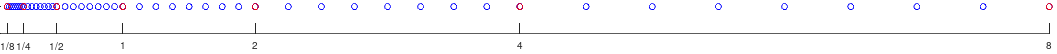
\includegraphics[scale=.4]{escala.png}
\caption{Algunos números positivos de máquina con $b=2$ y $m=4$. Notar que los números son equiespaciados únicamente entre potencias sucesivas de $2$, y que la cantidad de números de máquina en esos rangos se mantiene constante.}
\end{figure}
\begin{tcolorbox}{\bf Distribución de los números de máquina:}
Los números de máquina no se distribuyen de manera uniforme. Describamos dos números de máquina consecutivos  $x_1<x_2$ asumiendo, para simplificar,  que $0<x_1$ y que se escribe:
$$(x_1)_b= 0.b_0b_1b_2...b_{m-1}\, b^{e}.$$
Un momento de reflexión nos dice que el próximo número de máquina (salvo que haya overflow) será
$$(x_2)_b=0.b_0b_1b_2...(b_{m-1}+1)\, b^{e}$$
salvo que $b_{m-1}=b-1$ en cuyo caso
$$(x_2)_b=0.b_0b_1b_2...(b_{m-2}+1)0\, b^{e}$$
salvo que también $b_{m-2}=b-1$ en cuyo caso habrá que repetir el argumento y eventualmente -en caso de que $b_i=b-1$ para todo $0\le i\le m-1$
$$(x_2)_b=0.1b^{e+1}.$$
En cualquier caso observamos que
$$
x_2-x_1=b^{-m}b^e
$$
\emph{no es constante} al variar el exponente $e$, pero sí lo es para cada exponente fijo dado.

\end{tcolorbox}

La consecuencia mas notable de la distribución de los números de máquina es que si $x\in \R$, y existen $x_1<x_2$ números de máquina tales que $x_1\le x\le x_2$ (i.e. $x$ esta dentro de las escalas manejadas por la máquina) entonces
$$
|x-fl_{redond}(x)|\le \frac12 b^{e-m}
$$
$$
|x-fl_{trunc}(x)|\le b^{e-m}
$$
para los casos de redondeo y truncado respectivamente.
\begin{tcolorbox}{\bf Error relativo y precisión de la máquina:}
Nos concentraremos en el caso de redondeo, por lo que asumiremos de aquí en mas que  $fl=fl_{redond}$. Queremos acotar el error relativo al almacenar un número $x\neq 0$.  Observando que
$$b^{e-1}=|0.1\, b^{e}|\le  |x|,$$
resulta
$$
|\frac{x-fl(x)}{x}|\le \frac12 b^{1-m}.
$$
Notar que el error relativo depende \emph{del tamaño de la mantisa}. En el caso de base $b=2$ y $m=52$ mencionado antes resulta:
$$
|\frac{x-fl(x)}{x}|\le  2^{-52}\sim 10^{-16}.
$$
este número, propio de cada máquina, se denomina: precisión de la máquina o épsilon de la máquina y se denota con $\varepsilon$.

En el caso del ejemplo, en terminos simples, dice que nuestra máquina almacena 16 dígitos exactos (en base 10). Naturalemente sería ideal conservar esta precisión a lo largo de las  operaciones que debamos realizar a partir de  $fl(x)$. Eso, como veremos a continuación,  no es posible en general.
\end{tcolorbox}

Como acabamos de ver, en general ocurre que
$x\neq fl(x)$\footnote{Notemos que incluso números muy sencillos como $\frac{1}{10}$ no son de máquina y la introducción de un error de redondeo es inevitable. Evalúe en Python la expresión
$0.1+0.1+0.1!=0.3$, qué obtiene?.}. . Sin embargo podemos garantizar que la diferencia verifica
$$
x-fl(x)=\mu_x x,
$$
con
$$
\frac{|x-fl(x)|}{|x|} =|\mu_x|\le \varepsilon.
$$
Veamos entonces que ocurre con estos errores al efectuar alguna operación
sencilla como por ejemplo sumar. Vamos a distinguir la operación realizada por la máquina con el símbolo $\oplus$.

Pretendemos calcular $x+y$, de modo simplificado la máquina realiza las siguientes operaciones: primero
$$
x\to fl(x) \qquad y\to fl(y)
$$
luego suma $fl(x)+fl(y)$ y finalmente almacena el resultado
$$
fl(x)+fl(y)\to fl(fl(x)+fl(y)).
$$
Cómo se comportará el error resultante?.
Por una lado tenemos:
$$fl(x)=x(1+\mu_x),\qquad  fl(y)=y(1+\mu_y
y),$$ por lo que
$$fl(fl(x)+fl(y))=(fl(x)+fl(y))(1+\mu_z)$$
y en definitiva
$$
x\oplus y =fl(fl(x)+fl(y))=(x(1+\mu_x)+y(1+\mu_y
y))(1+\mu_z).
$$
Vemos entonces que \emph{si $0<x,y$} es posible acotar
$$
|x\oplus y -(x+y)|\le (x+y)2\mu +O(\varepsilon^2)
$$
con $|\mu|\le \varepsilon$. Es decir que hemos de algún modo preservado el tamaño del error relativo\footnote{Cuando los errores se acumulan de forma aditiva, como en este caso, estamos en un buen escenario porque harían falta una enorme cantidad de operaciones para deteriorar el error inicial.}  Como es  bien sabido, eso no es posible si \emph{restamos}
números similares\footnote{Verifique que la cuenta anterior no puede repetirse si los signos de $x$ e $y$ difieren.}.
Un ejemplo elemental es el siguiente: tomemos $b=10$, $m=4$, la precisión es $\varepsilon=\frac{1}{2}10^{-3}=0.0005$. Si $x=125,49$ e $y=125,31$ tenemos respectivamente
$x-y=0.18$
$x\ominus y=0.2$ por lo que el error relativo es
$$
|\frac{x-y-x\ominus y}{x-y}|=\frac{0.02}{0.18}\sim 0.11,
$$
es decir que a pesar de que $\varepsilon \sim 10^{-3}$ el error en la cuenta anterior es del $11\%$. El ejemplo anterior muestra que en una simple operación podemos perder dígitos significativos (de hecho nuestra máquina no ha acertado ningún dígito de la solución). Como regla general deben evitarse restas de números similares\footnote{Ver la guía de ejercicios para mas ejemplos} para evitar la denominada \emph{cancelación catastrófica}.

Es fácil construir ejemplos de números de máquina $0<x<y$ en los cuales no solo $x+y\neq x\oplus y$ sino que, por ejemplo, $x\oplus y=y$. En particular es fácil ver que
\begin{equation}
 \label{eq:epsilonmasuno}
 1 \oplus\varepsilon> 1,
\end{equation}
y
$$
1\oplus\varepsilon/2=1
$$
lo que da una posible definición alternativa del $\epsilon$ como el menor número de máquina con la  propiedad \eqref{eq:epsilonmasuno}.
Otras cuestión que aparece entonces en la aritmética de la máquina es la pérdida de la propiedad asociativa, ya que usando los comentarios previos vemos que por ejemplo
$$
(1\oplus \varepsilon/2)\oplus \varepsilon/2=1\neq 1\oplus (\varepsilon/2+\varepsilon/2).
$$

Hay diversas fuentes de errores computacionales que pueden estropear completamente el resultado de los algoritmos. En este sentido hay dos conceptos que nombraremos tangencialmente ya que no son objeto central de este curso: la \emph{condición} y la \emph{estabilidad}.

\section{Condición y estabilidad}
De manera muy general, un \emph{problema bien condicionado} es aquél que reacciona benignamente con los errores en los datos. Es decir, que sus soluciones no varían demasiado al no variar demasiado los datos. Por el contrario, si un problema está muy mal condicionado, no lograremos resolverlo con mucha precisión aunque limitemos los errores en los datos (salvo que trabajemos con precisión infinita). La noción de condición es algo \emph{intrínseco del problema} y está mas allá de nuestro algoritmo de resolución.  Por otra parte, cuando los problemas están bien condicionados tenemos esperanza de resolverlos con precisión siempre que nuestro algoritmo no incremente desproporcionadamente los errores inherentes a los datos. En este caso hablaramos de \emph{algoritmos estables} y por el contrario, de  \emph{algoritmos inestables} si no cumplen con este criterio. La estabilidad entonces es algo \emph{intrínseco del algoritmo}.




\begin{tcolorbox}
Es posible dar una expresión precisa para la noción de condición, a través del llamado
\emph{número de condición}. Consideremos el problema de evaluar una función en el valor $x_0\neq 0$. Si por alguna razón (error de medición o redondeo) modificamos el dato a evaluar $x_0$ en un una cierta magnitud pequeña $h$ entonces el error relativo que cometeremos es (asumiendo que la función es de continuamente diferenciable)
$$
\frac{f(x_0+h)-f(x_0)}{f(x_0)}=
\frac{hf'(\eta)}{f(x_0)},$$
para cierto $\eta$ intermedio entre $x_0$ y $x_0+h$. Esto indica que para $h\sim 0$
$$
\frac{hf'(\eta)}{f(x_0)}\sim
\frac{x_0f'(x_0)}{f(x_0)}\frac{h}{x_0}
$$
el error relativo en los datos $\frac{h}{x_0}$ se magnifica en nuestro problema en un factor
$$
\frac{|x_0||f'(x_0)|}{|f(x_0)|},
$$
llamado el \emph{número de condición} de evaluar $f$ en $x_0$. Siguiendo un razonamiento similar vemos que para la versión $f:\Rn\to \Rm$ puede definirse el número de condición de este problema de la forma\footnote{Un ejemplo concreto y elemental de mal condicionamiento es, como hemos visto, la resta de números similares: si escribimos
$f:\R^2\to \R$, $f(x,y)=x-y$, se tiene $Df(x_0,y_0)=(1,-1)$, $\|(1,-1)\|_{\infty}=2$, $\|(x_0,y_0)\|_{\infty}=max\{|x_0|,|y_0|\}$, luego $\frac{\|x_0\|\|Df(x_0)\|}{\|f(x_0)\|}\sim \frac{1}{\|x_0-y_0\|}.$}
\end{tcolorbox}
Como ejemplo de lo anterior
si queremos evaluar $tg(x)$ en un $x_0<\pi/2$, $x_0\sim \pi/2$ vemos que el número de condición
$$
\frac{x_0}{sen(x_0)cos(x_0)},
$$
cumple que
$$
\lim_{x_0\to \pi/2^-} \frac{x_0}{sen(x_0)cos(x_0)}=+\infty.
$$
En particular si elegimos  $x_0$ tal que $\frac{x_0}{sen(x_0)cos(x_0)}\sim 10^{16}$ no esperamos tener ningún dígito significativo en nuestro cálculo de $tg(x_0)$.
%\footnote{Paul Olum, sabiendo que a su amigo Feynmann le gustaba sorprender a todos haciendo cálculos mentales, le pidió un día que aproximara mentalmente $tg(10^{100})$. Feynmann supo al instante que estaba condenado.}.


En los años 50, Wilkinson experimentaba con las primeras computadoras y rápidamente comenzó a observar fenomenos de inestabilidades y mal condicionamiento\footnote{En sus propias palabras: ``The cosy relationship that mathematics enjoyed with polynomials suffered a severe setback in the early fifities where electronic computers came into general use. Speaking for myself I regard it as the most traumatic experience in my carrer as a numerical analyst'' \cite{Wil}  }. Una cosa que notó, al probar un algoritmo de aproximación de raices, es que si al polinomio
$$
p(x)=\prod_{i=1}^{20}(x-i)
$$
se le perturba el coeficiente que acompaña a $x^{19}$ (cuyo valor es $210$ ) en $2^{-23}$ las raíces mayores a $7$ sufren considerables modificaciones. En particular las raices  $10,11,\dots 19$
se transforman en 5 pares complejos conjugados. Las $18$ y $19$ en complejos de la forma $19.5\dots\pm 19.5\dots i$, es decir que una perturbación de orden $2^{-23}$ genera variaciones de orden $1$. \footnote{A pesar de esto, se puede probar que las raíces dependen de forma continua respecto de los coeficientes.} Mostrando que el problema de calcular raices está muy mal condicionado.

Ejemplos de algoritmos inestables abundan. La inestabilidad es muy frecuente y se hace notar muy rápidamente porque los resultados obtenidos difieren notoriamente de lo esperado. Los casos mas extremos aparecen en procesos que deben iterarse en los cuales el error se acumula exponencialmente en vez de aditivamente. Sin embargo hay casos muy simples que pueden ejemplificarse.


Mas arriba vimos que restar números similares es un problema mal condicionado y por eso debe evitarse o tratarse con cautela.

Supongamos que queremos evaluar $e^{-12}$. Usando lo explicado mas arriba, podemos ver que se trata de un problema bien condicionado.  Si utilizamos un algoritmo basado en la serie convergente
$$
e^{-x}=1-x+\frac{1}{2!}x^2-\frac{1}{3!}x^3\cdots
$$
para una evaluación directa en $x=-12$ obtenemos, sumando los primeros 50 términos de la serie:
$$
e^{-12}\sim 6.144189436702122\cdot 10^{-6}.$$
Si por otro lado modificamos el algoritmo calculado primero $e^{12}$
sumando los primeros 50 terminos de la serie
$$
e^{x}=1+x+\frac{1}{2!}x^2+\frac{1}{3!}x^3\cdots
$$
y luego invirtiendo $1/e^{12}$ obtenemos
$$e^{-12}\sim 6.144212353328213\cdot 10^{-6}.$$
La pregunta es a priori, cuál de las dos respuestas es mas confiable. Sin duda el segundo método es mas estable. La razón es que en el cómputo de la serie alternada, muchos terminos ``grandes'' deben cancelarse mágicamente para producir el resultado ``pequeño'' $e^{-12}$. Los errores relativos pequeños son proporcionalmente grandes en términos del resultado final. De hecho
$$e^{-12}\sim 6.1442123533282097586823081788055323112239893148882529755...\cdot 10^{-6}$$
es decir que solo obtuvimos $4$ dígitos correctos con nuestro primero algoritmo pero $14$ con el segundo.
El segundo método es mucho mas estable que el primero. Puede probar los calculos previos con el algoritmo:

\begin{Shaded}
\begin{lstlisting}[language=python]
import numpy as np
import math
v=np.arange(0,50)
resulI=0.0
resulE=0.0
for i in v:
	resulI=resulI+1/math.factorial(i)*(-12.0)**i
	resulE=resulE+1/math.factorial(i)*(12.0)**i
resulE=1/resulE
print(resulInes)
print(resulEs)
\end{lstlisting}
\end{Shaded}
Los problemas que emergen debido a la precisión limitada de las máquinas dan lugar a muchos comportamientos inesperados. El ejemplo que damos a continuación, debido a Cleve Moler, es particularmente sencillo y sigue las consideraciones del ejemplo previo. Queremos evaluar $p(x)=(x-1)^7$ para posteriormente graficarlo.
En el primer algoritmo usamos la expresión cerrada $(x-1)^7$  y en el segundo método la expresión equivalente
$$
p(x)=x^7-7x^6+21x^5-35x^4+35x^3-21x^2+7x-1.
$$
En la Figura \ref{fig:moler} a la izquierda vemos ambos gráficos perfectamente superpuestos (azul para el primer método tapado por el rojo del segundo método).
\begin{figure}
 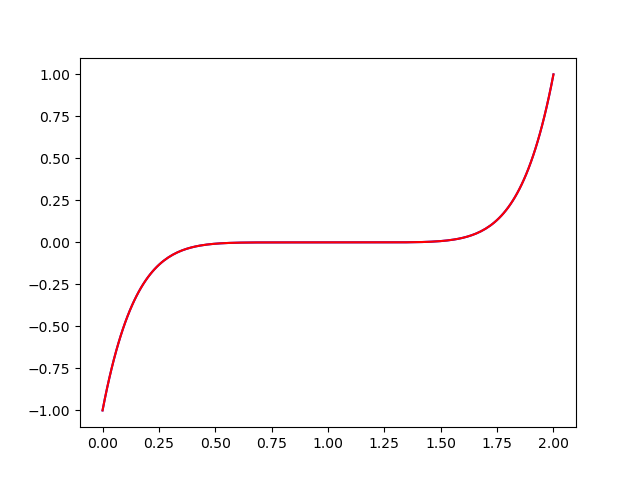
\includegraphics[scale=0.4]{moler1}
 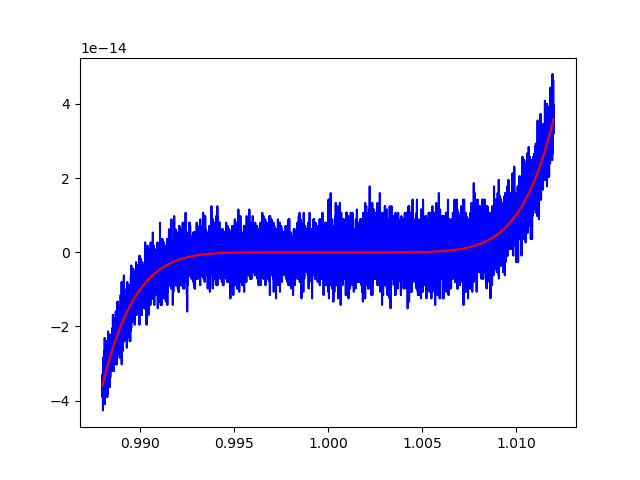
\includegraphics[scale=0.4]{moler2}
 \caption{Gráficos de $p(x)$}
 \label{fig:moler}
 \end{figure}
Sin embargo en la misma figura a la derecha se muestra un zoom cerca de la raíz del polinomio.

\begin{Shaded}
\begin{lstlisting}[language=python]
import numpy as np
import matplotlib.pyplot as plt
x=np.linspace(0,2,200)
plt.plot(x,x**7-7*x**6+21*x**5-35*x**4+35*x**3-21*x**2+7*x-1,'b', x,(x-1)**7,'r')
plt.show()

# Sin embargo a la derecha vemos el resultado de samplear en una
#escala mas fina alrededor de la raíz

x=np.linspace(0.988,1.012,10000)
plt.plot(x,x**7-7*x**6+21*x**5-35*x**4+35*x**3-21*x**2+7*x-1,'b', x,(x-1)**7,'r')
plt.show()
\end{lstlisting}
\end{Shaded}


Las nociones de condición y estabilidad que hemos comentado de modo superficial son temas transversales a toda el área del análisis  numérico. Como nos restringiremos a cuestiones de álgebra lineal solo hemos pretendido dar una idea somera de sus implicaciones generales. En el capítulo siguiente retomaremos la cuestión de la condición en el ámbito matricial.

